\documentclass[tikz,border=4pt]{standalone}
\usepackage[T1]{fontenc}
\usepackage{lmodern}
\renewcommand{\familydefault}{\sfdefault}
\usetikzlibrary{shapes.geometric,positioning,arrows.meta,calc,fit,backgrounds,decorations.pathreplacing}
\tikzset{
  node distance=6mm,
  every node/.style={font=\footnotesize,align=center,execute at begin node={\hyphenpenalty=10000\relax}},
  base/.style={draw=gray!60,fill=gray!12,minimum height=7mm,inner sep=2pt},
  term/.style={base,rounded corners=3.5mm,text width=30mm},
  proc/.style={base,text width=32mm},
  err/.style={base,text width=30mm,fill=gray!22},
  io/.style={base,trapezium,trapezium left angle=72,trapezium right angle=108,trapezium stretches=true,text width=28mm},
  dec/.style={base,diamond,aspect=2.4,text width=27mm,inner sep=0pt},
  % predefined process: a call to another procedure
  sub/.style={proc,inner xsep=3mm,path picture={
    \draw[gray!60] ([xshift=1.5mm]path picture bounding box.north west)--([xshift=1.5mm]path picture bounding box.south west)
                   ([xshift=-1.5mm]path picture bounding box.north east)--([xshift=-1.5mm]path picture bounding box.south east);}},
  go/.style={-{Stealth[length=2mm]},draw=gray!55!black},
  lab/.style={font=\scriptsize,fill=white,inner sep=1pt},
  frame/.style={draw=gray!60,dashed,rounded corners=2mm,inner sep=3mm},
  % memory diagrams
  cell/.style={draw=gray!60,fill=gray!12,minimum height=7mm,inner sep=1pt,font=\scriptsize},
  hot/.style={cell,fill=gray!35},
  note/.style={font=\scriptsize,text=gray!30!black},
}

\begin{document}
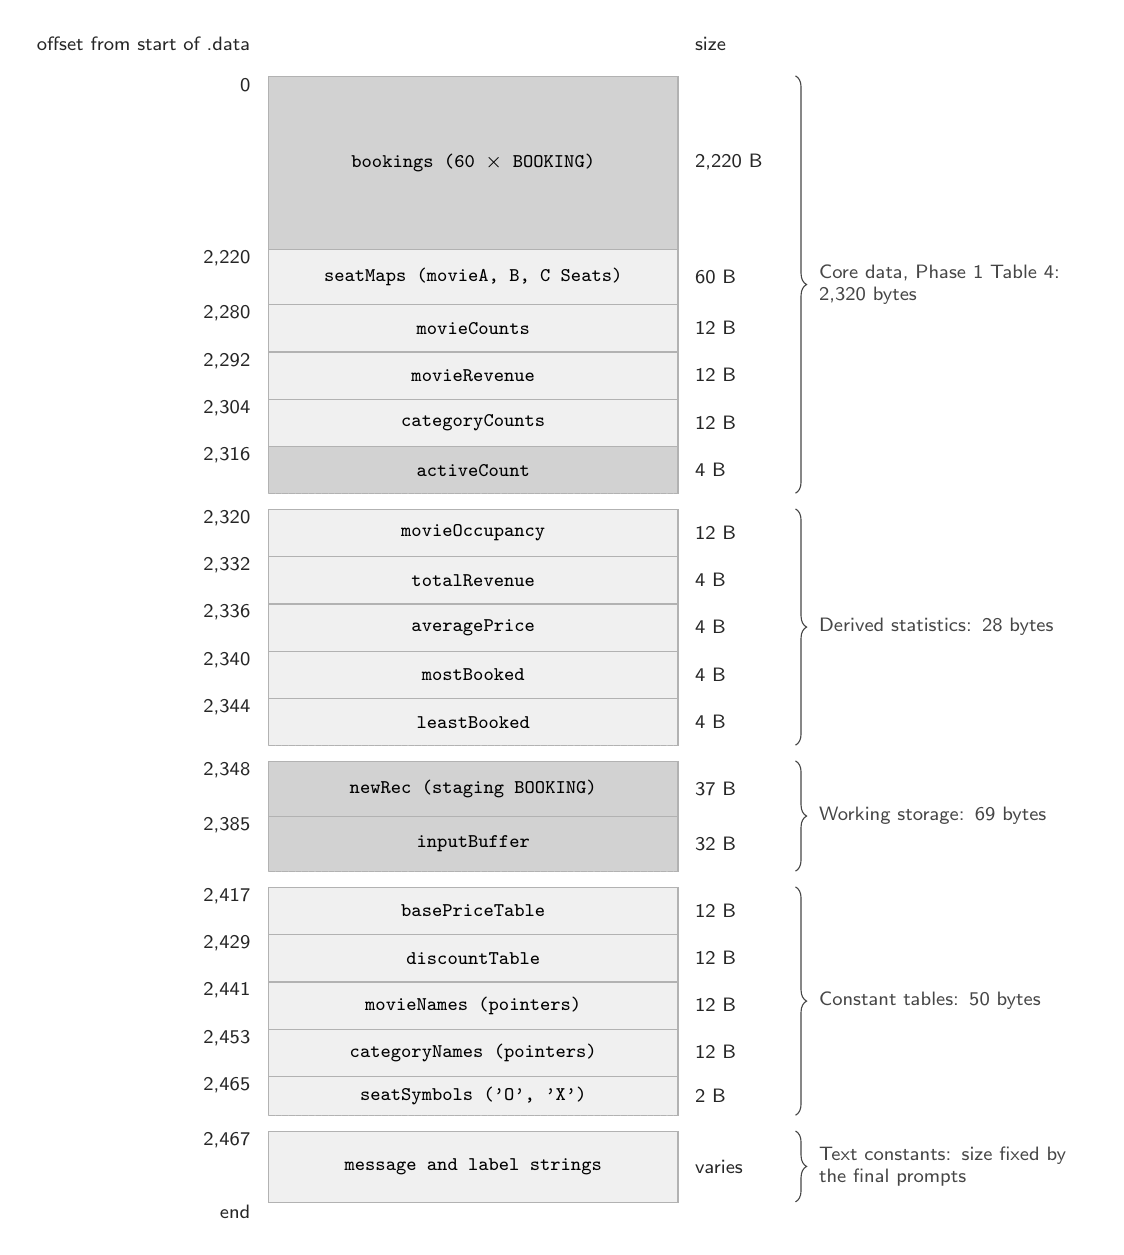
\begin{tikzpicture}[x=1mm,y=1mm]
\def\w{52}
% y position (top), height, offset, name, size, style
\foreach \y/\h/\off/\n/\sz/\st in {
  0/22/0/bookings (60 $\times$ BOOKING)/{2,220 B}/hot,
  -22/7/{2,220}/{seatMaps (movieA, B, C Seats)}/60 B/cell,
  -29/6/{2,280}/movieCounts/12 B/cell,
  -35/6/{2,292}/movieRevenue/12 B/cell,
  -41/6/{2,304}/categoryCounts/12 B/cell,
  -47/6/{2,316}/activeCount/4 B/hot,
  -55/6/{2,320}/movieOccupancy/12 B/cell,
  -61/6/{2,332}/totalRevenue/4 B/cell,
  -67/6/{2,336}/averagePrice/4 B/cell,
  -73/6/{2,340}/mostBooked/4 B/cell,
  -79/6/{2,344}/leastBooked/4 B/cell,
  -87/7/{2,348}/newRec (staging BOOKING)/37 B/hot,
  -94/7/{2,385}/inputBuffer/32 B/hot,
  -103/6/{2,417}/basePriceTable/12 B/cell,
  -109/6/{2,429}/discountTable/12 B/cell,
  -115/6/{2,441}/movieNames (pointers)/12 B/cell,
  -121/6/{2,453}/categoryNames (pointers)/12 B/cell,
  -127/5/{2,465}/{seatSymbols ('O', 'X')}/2 B/cell,
  -134/9/{2,467}/message and label strings/varies/cell}{
  \node[\st,minimum width=\w mm,minimum height=\h mm,anchor=north west] at (0,\y) {\texttt{\n}};
  \node[note,anchor=east] at (-1,\y-1.2) {\off};
  \node[note,anchor=west] at (\w+1,\y-\h/2) {\sz};}
\node[note,anchor=east] at (-1,-144.2) {end};
\node[note,anchor=south east] at (-1,2) {offset from start of .data};
\node[note,anchor=south west] at (\w+1,2) {size};
% group braces
\foreach \t/\b/\lab in {0/-53/{Core data, Phase 1 Table 4: 2,320 bytes},-55/-85/{Derived statistics: 28 bytes},-87/-101/{Working storage: 69 bytes},-103/-132/{Constant tables: 50 bytes},-134/-143/{Text constants: size fixed by the final prompts}}{
  \draw[decorate,decoration={brace,amplitude=4pt},gray!55!black] (\w+15,\t)--(\w+15,\b) node[midway,right=5pt,font=\scriptsize,align=left,text width=34mm]{\lab};}
% gap markers
\foreach \y in {-53,-85,-101,-132}{\draw[gray!50,dotted] (0,\y)--(\w,\y);}
\end{tikzpicture}
\end{document}
